\begin{problem}[Triangle Inequality and Cauchy-Schwarz]
For point $P(x,y,z)$ on unit sphere centered at origin, prove: (i) $|x| + |y| + |z| \geq 1$, (ii) Cauchy-Schwarz inequality, (iii) $|x| + |y| + |z| \leq \sqrt{3}$.
\end{problem}

\begin{hint}
Use triangle inequality for part (i) and Cauchy-Schwarz with vector $(1,1,1)$ for part (iii).
\end{hint}

\begin{solution}[Sketch]
(i) By triangle inequality: $1 = |\mathbf{r}| \leq |x| + |y| + |z|$. (ii) From dot product: $|\mathbf{a} \cdot \mathbf{b}| \leq |\mathbf{a}||\mathbf{b}|$. (iii) Apply Cauchy-Schwarz with $\mathbf{a} = (|x|,|y|,|z|)$, $\mathbf{b} = (1,1,1)$: $|x| + |y| + |z| \leq \sqrt{x^2+y^2+z^2}\sqrt{3} = \sqrt{3}$.
\end{solution}

\vspace{1em}

\begin{problem}[Bimedians of Tetrahedron]
On the triangular pyramid (tetrahedron) $ABCD$, let:
\begin{itemize}
    \item $L$ is the midpoint of $AB$
    \item $M$ is the midpoint of $AC$
    \item $N$ is the midpoint of $AD$
    \item $P$ is the midpoint of $CD$
    \item $Q$ is the midpoint of $BD$
    \item $R$ is the midpoint of $BC$
\end{itemize}

\begin{center}
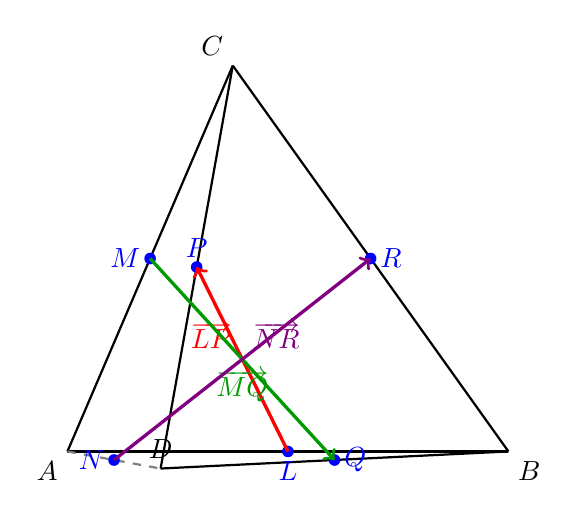
\begin{tikzpicture}[scale=1.4, line join=round]
    % Define vertices of tetrahedron
    \coordinate (A) at (0,0,0);
    \coordinate (B) at (4,0,0);
    \coordinate (C) at (1.5,3.5,0);
    \coordinate (D) at (2,1,3);
    
    % Calculate midpoints
    \coordinate (L) at (2,0,0);      % midpoint of AB
    \coordinate (M) at (0.75,1.75,0);  % midpoint of AC
    \coordinate (N) at (1,0.5,1.5);    % midpoint of AD
    \coordinate (P) at (1.75,2.25,1.5); % midpoint of CD
    \coordinate (Q) at (3,0.5,1.5);    % midpoint of BD
    \coordinate (R) at (2.75,1.75,0);  % midpoint of BC
    
    % Draw edges of tetrahedron (some dashed for hidden edges)
    \draw[thick] (A) -- (B);
    \draw[thick] (A) -- (C);
    \draw[thick, dashed, gray] (A) -- (D);
    \draw[thick] (B) -- (C);
    \draw[thick] (B) -- (D);
    \draw[thick] (C) -- (D);
    
    % Draw midpoints
    \fill[blue] (L) circle (1.5pt);
    \fill[blue] (M) circle (1.5pt);
    \fill[blue] (N) circle (1.5pt);
    \fill[blue] (P) circle (1.5pt);
    \fill[blue] (Q) circle (1.5pt);
    \fill[blue] (R) circle (1.5pt);
    
    % Draw bimedian vectors
    \draw[->, very thick, red] (L) -- (P) node[midway, above left, red] {$\overrightarrow{LP}$};
    \draw[->, very thick, green!60!black] (M) -- (Q) node[midway, below, green!60!black] {$\overrightarrow{MQ}$};
    \draw[->, very thick, violet] (N) -- (R) node[midway, above right, violet] {$\overrightarrow{NR}$};
    
    % Label vertices
    \node[below left] at (A) {$A$};
    \node[below right] at (B) {$B$};
    \node[above left] at (C) {$C$};
    \node[above] at (D) {$D$};
    
    % Label midpoints
    \node[below, blue] at (L) {$L$};
    \node[left, blue] at (M) {$M$};
    \node[left, blue] at (N) {$N$};
    \node[above, blue] at (P) {$P$};
    \node[right, blue] at (Q) {$Q$};
    \node[right, blue] at (R) {$R$};
\end{tikzpicture}
\end{center}

\textit{Note: The three colored arrows show the bimedians $\overrightarrow{LP}$ (red), $\overrightarrow{MQ}$ (green), and $\overrightarrow{NR}$ (violet). Each bimedian connects the midpoint of one edge to the midpoint of the opposite edge.}

Let $\mathbf{b} = \overrightarrow{AB}$, $\mathbf{c} = \overrightarrow{AC}$ and $\mathbf{d} = \overrightarrow{AD}$.

\begin{enumerate}[label=(\roman*)]
    \item Show that $\overrightarrow{LP} = \frac{1}{2}(-\mathbf{b} + \mathbf{c} + \mathbf{d})$.
    
    \item It can be shown that:
    \[
    \overrightarrow{MQ} = \frac{1}{2}(\mathbf{b} - \mathbf{c} + \mathbf{d}) \quad \text{and} \quad \overrightarrow{NR} = \frac{1}{2}(\mathbf{b} + \mathbf{c} - \mathbf{d})
    \]
    (Do NOT prove these.)
    
    Prove that:
    \[
    |AB|^2 + |AC|^2 + |AD|^2 + |BC|^2 + |BD|^2 + |CD|^2 = 4\left( |LP|^2 + |MQ|^2 + |NR|^2 \right)
    \]
\end{enumerate}

\textit{Note: The segments $LP$, $MQ$, and $NR$ are called the bimedians of the tetrahedron. This problem proves that the sum of the squares of all six edges equals four times the sum of the squares of the three bimedians.}
\end{problem}

\begin{hint}
(i) Express $\overrightarrow{AL}$ and $\overrightarrow{AP}$ in terms of $\mathbf{b}$, $\mathbf{c}$, and $\mathbf{d}$, then find $\overrightarrow{LP} = \overrightarrow{AP} - \overrightarrow{AL}$.
(ii) Expand the left side as the sum of squared magnitudes of all six edges. Expand the right side by computing $4|LP|^2$, $4|MQ|^2$, and $4|NR|^2$ using dot products. Show both sides equal $3(b^2 + c^2 + d^2) - 2(\mathbf{b}\cdot\mathbf{c} + \mathbf{b}\cdot\mathbf{d} + \mathbf{c}\cdot\mathbf{d})$.
\end{hint}

\begin{solution}[Sketch]
(i) Since $L$ is midpoint of $AB$: $\overrightarrow{AL} = \frac{1}{2}\mathbf{b}$. Since $P$ is midpoint of $CD$: $\overrightarrow{AP} = \frac{1}{2}(\mathbf{c} + \mathbf{d})$. Therefore: $\overrightarrow{LP} = \overrightarrow{AP} - \overrightarrow{AL} = \frac{1}{2}(\mathbf{c} + \mathbf{d}) - \frac{1}{2}\mathbf{b} = \frac{1}{2}(-\mathbf{b} + \mathbf{c} + \mathbf{d})$.

(ii) LHS: The six edges are $AB$, $AC$, $AD$, $BC = \mathbf{c}-\mathbf{b}$, $BD = \mathbf{d}-\mathbf{b}$, $CD = \mathbf{d}-\mathbf{c}$.
\begin{align*}
LHS &= |\mathbf{b}|^2 + |\mathbf{c}|^2 + |\mathbf{d}|^2 + |\mathbf{c}-\mathbf{b}|^2 + |\mathbf{d}-\mathbf{b}|^2 + |\mathbf{d}-\mathbf{c}|^2 \\
&= 3(b^2 + c^2 + d^2) - 2(\mathbf{b}\cdot\mathbf{c} + \mathbf{b}\cdot\mathbf{d} + \mathbf{c}\cdot\mathbf{d})
\end{align*}

RHS: Using part (i) and the given expressions:
\begin{align*}
4|LP|^2 &= b^2 + c^2 + d^2 - 2\mathbf{b}\cdot\mathbf{c} - 2\mathbf{b}\cdot\mathbf{d} + 2\mathbf{c}\cdot\mathbf{d} \\
4|MQ|^2 &= b^2 + c^2 + d^2 - 2\mathbf{b}\cdot\mathbf{c} + 2\mathbf{b}\cdot\mathbf{d} - 2\mathbf{c}\cdot\mathbf{d} \\
4|NR|^2 &= b^2 + c^2 + d^2 + 2\mathbf{b}\cdot\mathbf{c} - 2\mathbf{b}\cdot\mathbf{d} - 2\mathbf{c}\cdot\mathbf{d}
\end{align*}

Summing: $RHS = 3(b^2 + c^2 + d^2) - 2(\mathbf{b}\cdot\mathbf{c} + \mathbf{b}\cdot\mathbf{d} + \mathbf{c}\cdot\mathbf{d}) = LHS$.
\end{solution}

\vspace{1em}

\begin{problem}[Triangle Intersection Ratios]
The diagram shows triangle $OQA$.

The point $P$ lies on $OA$ so that $OP : OA = 3 : 5$.

The point $B$ lies on $OQ$ so that $OB : OQ = 1 : 3$.

The point $R$ is the intersection of $AB$ and $PQ$.

The point $T$ is chosen on $AQ$ so that $O, R$ and $T$ are collinear.

Let $\mathbf{a} = \overrightarrow{OA}$, $\mathbf{b} = \overrightarrow{OB}$ and $\overrightarrow{PR} = k\overrightarrow{PQ}$ where $k$ is a real number.

\begin{enumerate}[label=(\roman*)]
    \item Show that $\overrightarrow{OR} = \frac{3}{5}(1-k)\mathbf{a} + 3k\mathbf{b}$.
    
    \item Writing $\overrightarrow{AR} = h\overrightarrow{AB}$, where $h$ is a real number, it can be shown that $\overrightarrow{OR} = (1-h)\mathbf{a} + h\mathbf{b}$. (Do NOT prove this.)
    
    Show that $k = \frac{1}{6}$.

    \item Find $\overrightarrow{OT}$ in terms of $\mathbf{a}$ and $\mathbf{b}$.
\end{enumerate}
\end{problem}

\begin{hint}
(i) Express $\overrightarrow{OR}$ as $\overrightarrow{OP} + \overrightarrow{PR}$. Use $\overrightarrow{OP} = \frac{3}{5}\mathbf{a}$ and $\overrightarrow{PQ} = -\overrightarrow{OP} + \overrightarrow{OQ}$ where $\overrightarrow{OQ} = 3\mathbf{b}$.
(ii) Equate coefficients of $\mathbf{a}$ and $\mathbf{b}$ from the two expressions for $\overrightarrow{OR}$. Use the relationship $3k = h$ and solve the system.
(iii) Since $O, R, T$ are collinear: $\overrightarrow{OT} = \lambda\overrightarrow{OR}$. Since $T$ is on $AQ$: $\overrightarrow{OT} = (1-\mu)\mathbf{a} + 3\mu\mathbf{b}$. Equate coefficients.
\end{hint}

\begin{solution}[Sketch]
(i) $\overrightarrow{OR} = \overrightarrow{OP} + k\overrightarrow{PQ}$. Since $\overrightarrow{OP} = \frac{3}{5}\mathbf{a}$ and $\overrightarrow{OQ} = 3\mathbf{b}$, we have:
$\overrightarrow{PQ} = -\frac{3}{5}\mathbf{a} + 3\mathbf{b}$.
Therefore: $\overrightarrow{OR} = \frac{3}{5}\mathbf{a} + k(-\frac{3}{5}\mathbf{a} + 3\mathbf{b}) = \frac{3}{5}(1-k)\mathbf{a} + 3k\mathbf{b}$.

(ii) Equating coefficients from both expressions:
For $\mathbf{b}$: $3k = h$.
For $\mathbf{a}$: $\frac{3}{5}(1-k) = 1-h$.
Substitute $h = 3k$ into second equation: $\frac{3}{5}(1-k) = 1-3k \Rightarrow 3(1-k) = 5(1-3k) \Rightarrow 3-3k = 5-15k \Rightarrow 12k = 2 \Rightarrow k = \frac{1}{6}$.

(iii) From part (ii): $\overrightarrow{OR} = \frac{3}{5}(1-\frac{1}{6})\mathbf{a} + 3(\frac{1}{6})\mathbf{b} = \frac{1}{2}\mathbf{a} + \frac{1}{2}\mathbf{b}$.

Since $O, R, T$ collinear: $\overrightarrow{OT} = \lambda\overrightarrow{OR} = \frac{\lambda}{2}(\mathbf{a} + \mathbf{b})$.

Since $T$ on $AQ$: $\overrightarrow{OT} = \mathbf{a} + \mu(\overrightarrow{OQ} - \mathbf{a}) = (1-\mu)\mathbf{a} + 3\mu\mathbf{b}$.

Equating coefficients: $\frac{\lambda}{2} = 1-\mu$ and $\frac{\lambda}{2} = 3\mu$.
From these: $1-\mu = 3\mu \Rightarrow \mu = \frac{1}{4}$.
Therefore: $\overrightarrow{OT} = (1-\frac{1}{4})\mathbf{a} + 3(\frac{1}{4})\mathbf{b} = \frac{3}{4}\mathbf{a} + \frac{3}{4}\mathbf{b} = \frac{3}{4}(\mathbf{a} + \mathbf{b})$.
\end{solution}

\vspace{1em}

\begin{problem}[Circle Intersection of Sets]
Let $A$ and $B$ be two distinct points in three-dimensional space. Let $M$ be the midpoint of $AB$.

Let $S_1$ be the set of all points $P$ such that $\overrightarrow{AP} \cdot \overrightarrow{BP} = 0$.

Let $S_2$ be the set of all points $N$ such that $\left| \overrightarrow{AN} \right| = \left| \overrightarrow{MN} \right|$.

The intersection of $S_1$ and $S_2$ is the circle $S$.

What is the radius of the circle $S$?

\begin{enumerate}[label=\Alph*.]
    \item $\displaystyle \frac{\left| \overrightarrow{AB} \right|}{2}$
    \item $\displaystyle \frac{\left| \overrightarrow{AB} \right|}{4}$
    \item $\displaystyle \frac{\sqrt{3} \left| \overrightarrow{AB} \right|}{2}$
    \item $\displaystyle \frac{\sqrt{3} \left| \overrightarrow{AB} \right|}{4}$
\end{enumerate}
\end{problem}

\begin{hint}
(Step 1) Recognize that $\overrightarrow{AP} \cdot \overrightarrow{BP} = 0$ defines a sphere with diameter $AB$ centered at $M$. (Step 2) The condition $|\overrightarrow{AN}| = |\overrightarrow{MN}|$ describes the perpendicular bisecting plane of segment $AM$. (Step 3) Use the Pythagorean relationship $r^2 + d^2 = R_{sphere}^2$ where $d$ is the distance from the sphere center to the plane.
\end{hint}

\begin{solution}[Sketch]
\textbf{Step 1: Analyze set $S_1$.} The condition $\overrightarrow{AP} \cdot \overrightarrow{BP} = 0$ means vectors $\overrightarrow{AP}$ and $\overrightarrow{BP}$ are perpendicular. The locus of points $P$ that subtend a right angle to segment $AB$ is a sphere with diameter $AB$. Center: $M$ (midpoint of $AB$). Radius: $R_{sphere} = \frac{1}{2}|\overrightarrow{AB}|$.

\textbf{Step 2: Analyze set $S_2$.} The condition $|\overrightarrow{AN}| = |\overrightarrow{MN}|$ describes points equidistant from $A$ and $M$, which is the perpendicular bisecting plane of segment $AM$.

\textbf{Step 3: Find intersection.} The intersection of a sphere (centered at $M$) and a plane is a circle. Using the Pythagorean relationship: $r^2 + d^2 = R_{sphere}^2$ where $d$ is the perpendicular distance from center $M$ to the plane.

\textbf{Step 4: Calculate distances.} Since the plane passes through the midpoint of $AM$, and $|\overrightarrow{AM}| = \frac{1}{2}|\overrightarrow{AB}|$, we have:
\[ d = \frac{1}{2}|\overrightarrow{AM}| = \frac{1}{2} \left( \frac{1}{2}|\overrightarrow{AB}| \right) = \frac{1}{4}|\overrightarrow{AB}| \]

\textbf{Step 5: Solve for radius $r$.}
\begin{align*}
    r^2 &= R_{sphere}^2 - d^2 = \left( \frac{|\overrightarrow{AB}|}{2} \right)^2 - \left( \frac{|\overrightarrow{AB}|}{4} \right)^2 \\
    &= \frac{|\overrightarrow{AB}|^2}{4} - \frac{|\overrightarrow{AB}|^2}{16} = \frac{4|\overrightarrow{AB}|^2 - |\overrightarrow{AB}|^2}{16} = \frac{3|\overrightarrow{AB}|^2}{16} \\
    r &= \frac{\sqrt{3}|\overrightarrow{AB}|}{4}
\end{align*}

Therefore, the answer is \textbf{D}.
\end{solution}

\vspace{1em}

\begin{problem}[Complex Numbers and Centroid]
The complex numbers $x$, $w$, and $z$ are all different and all have modulus 1 (i.e., they lie on the unit circle in the complex plane).

The \textbf{centroid} (also called the center of mass) of three points is the average of their positions, given by $G = \frac{1}{3}(x + w + z)$.

Prove that $\frac{1}{3}(x + w + z)$ is never a cube root of $xwz$.

\textit{Note: A cube root of $xwz$ is any complex number $K$ satisfying $K^3 = xwz$.}
\end{problem}

\begin{hint}
Show that the centroid has modulus strictly less than 1 (using the triangle inequality with strict inequality since the points are distinct), while any cube root of $xwz$ has modulus exactly 1.
\end{hint}

\begin{solution}[Sketch]
Given: $|x| = |w| = |z| = 1$ and $x, w, z$ are all different.

\textbf{Step 1: Find modulus of any cube root.} Let $K$ be any cube root of $xwz$, so $K^3 = xwz$. Taking modulus: $|K|^3 = |xwz| = |x||w||z| = 1 \cdot 1 \cdot 1 = 1$. Therefore $|K| = 1$. Thus, any cube root of $xwz$ lies on the unit circle.

\textbf{Step 2: Find modulus of centroid.} The centroid is $G = \frac{1}{3}(x + w + z)$. By triangle inequality: $|x + w + z| \leq |x| + |w| + |z| = 3$. Equality holds only if $x, w, z$ have the same argument (same direction), which means $x = w = z$. But they are given to be different, so strict inequality holds: $|x + w + z| < 3$. Therefore: $|G| = \left|\frac{x + w + z}{3}\right| < 1$.

\textbf{Conclusion:} Since $|G| < 1$ but $|K| = 1$ for any cube root $K$, we have $G \neq K$. Therefore, the centroid is never a cube root of the product.
\end{solution}

\vspace{1em}

\begin{problem}[Parallelogram Intersection Ratio]
In parallelogram $OPQR$ with diagonals intersecting at $T$, prove $T$ divides diagonal $PR$ in ratio $2:1$.

\begin{center}
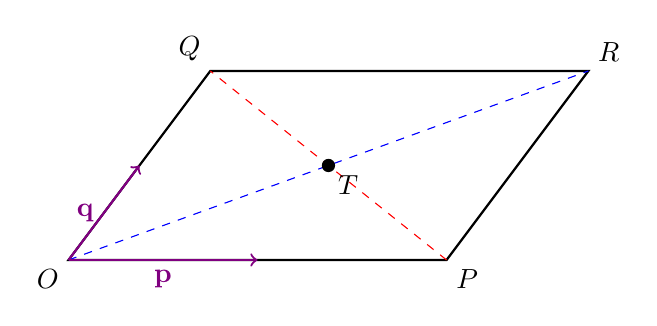
\begin{tikzpicture}[scale=1.2]
    % Define vertices
    \coordinate (O) at (0,0);
    \coordinate (P) at (4,0);
    \coordinate (Q) at (1.5,2);
    \coordinate (R) at (5.5,2);
    
    % Draw parallelogram
    \draw[thick] (O) -- (P) -- (R) -- (Q) -- cycle;
    
    % Draw diagonals
    \draw[dashed, blue] (O) -- (R);
    \draw[dashed, red] (P) -- (Q);
    
    % Calculate intersection point T (diagonals of parallelogram bisect each other)
    \coordinate (T) at (2.75,1);
    
    % Draw point T
    \fill[black] (T) circle (2pt);
    
    % Label vertices
    \node[below left] at (O) {$O$};
    \node[below right] at (P) {$P$};
    \node[above left] at (Q) {$Q$};
    \node[above right] at (R) {$R$};
    \node[below right] at (T) {$T$};
    
    % Optional: mark the vectors
    \draw[->, thick, violet] (O) -- (2,0) node[midway, below] {$\mathbf{p}$};
    \draw[->, thick, violet] (O) -- (0.75,1) node[midway, left] {$\mathbf{q}$};
\end{tikzpicture}
\end{center}

\textit{Note: In the diagram, $\mathbf{p} = \overrightarrow{OP}$ and $\mathbf{q} = \overrightarrow{OQ}$ (or equivalently $\mathbf{r} = \overrightarrow{OR}$). The diagonals OR and PQ intersect at point T.}
\end{problem}

\begin{hint}
Express $\overrightarrow{OT}$ via midpoint $S$ of $QR$ using collinearity, then via diagonal $PR$.
\end{hint>

\begin{solution}[Sketch]
Find $\overrightarrow{OS} = \mathbf{r} + \frac{1}{2}\mathbf{p}$. Since $T$ on $OS$: $\overrightarrow{OT} = \lambda(\mathbf{r} + \frac{\mathbf{p}}{2})$. Since $T$ on $PR$: coefficients sum to 1. Solve: $\lambda(\frac{1}{2}) + \lambda = 1 \Rightarrow \lambda = \frac{2}{3}$. Thus $\overrightarrow{OT} = \frac{2}{3}\mathbf{r} + \frac{1}{3}\mathbf{p}$, giving ratio $PT:TR = 2:1$.
\end{solution}

\vspace{1em}

\begin{problem}[Pyramid Centroid]
For pyramid with square base $ABCD$ and apex $S$, show sum of vectors from center of base to all vertices is zero, then find centroid $G$ of pyramid.
\end{problem}

\begin{hint}
Diagonals of square bisect at $H$. Use symmetry to show $\overrightarrow{HA} + \overrightarrow{HC} = \vec{0}$ and $\overrightarrow{HB} + \overrightarrow{HD} = \vec{0}$.
\end{hint}

\begin{solution}[Sketch]
(i) $H$ is midpoint of diagonals: $\overrightarrow{HA} = -\overrightarrow{HC}$ and $\overrightarrow{HB} = -\overrightarrow{HD}$, so sum is zero. (ii) From $\sum \overrightarrow{GA_i} = \vec{0}$, get $4\overrightarrow{GH} + \overrightarrow{GS} = \vec{0}$. Therefore $\overrightarrow{HG} = \frac{1}{5}\overrightarrow{HS}$, giving $\lambda = \frac{1}{5}$.
\end{solution}

\vspace{1em}

\begin{problem}[Point-to-Line Distance via Quadratic]
Show that $|\overrightarrow{AB}|^2 = 6p^2 - 24p + 125$ where $B$ is on line through origin. Find shortest distance from $A$ to line.
\end{problem}

\begin{hint}
Minimize the quadratic by completing the square or using calculus.
\end{hint}

\begin{solution}[Sketch]
Express $\overrightarrow{AB} = \begin{pmatrix} p-8 \\ p+6 \\ 2p-5 \end{pmatrix}$. Square and sum: $|\overrightarrow{AB}|^2 = (p-8)^2 + (p+6)^2 + (2p-5)^2 = 6p^2 - 24p + 125$. Complete square: $6(p-2)^2 + 101$. Minimum at $p=2$ gives $|\overrightarrow{AB}|_{\min}^2 = 101$, so distance $= \sqrt{101}$.
\end{solution}

\vspace{1em}

\begin{problem}[Triangle Intersection with Complex Centroid]
Points on triangle with various constructions. Show centroid lies on specific line and prove relationship.
\end{problem}

\begin{hint}
Express vectors through different routes and use coefficient uniqueness.
\end{hint}

\begin{solution}[Sketch]
Given $\overrightarrow{SK} = \frac{1}{4}\overrightarrow{SB} + \frac{1}{3}\overrightarrow{SC}$ and $L$ on $BC$. Show $\overrightarrow{OR} = \frac{1}{2}(\mathbf{a} + \mathbf{b})$ by expressing via paths through $P$ and $Q$. Find $k = \frac{1}{6}$. Centroid $G$ position: $\overrightarrow{OG} = \frac{1}{3}(\mathbf{a} + \mathbf{b} + \mathbf{c})$ lies on line $MC$ where $M$ is midpoint of $AB$.
\end{solution}

\vspace{1em}

\begin{problem}[Line-Sphere Intersection Points]
Find intersection points of line $\mathbf{r} = \mathbf{i} + 3\mathbf{j} - 4\mathbf{k} + t(\mathbf{i} + 2\mathbf{j} + 2\mathbf{k})$ and sphere $(x-1)^2 + (y-3)^2 + (z+4)^2 = 81$.
\end{problem}

\begin{hint}
Substitute parametric equations into sphere equation and solve resulting quadratic.
\end{hint}

\begin{solution}[Sketch]
Parametric: $x = 1+t$, $y = 3+2t$, $z = -4+2t$. Substitute: $(t)^2 + (2t)^2 + (2t)^2 = 81 \Rightarrow 9t^2 = 81 \Rightarrow t = \pm 3$. Points: $(4, 9, 2)$ when $t=3$ and $(-2, -3, -10)$ when $t=-3$.
\end{solution}

\vspace{1em}

\begin{problem}[Line Tangent to Sphere]
Show line intersects sphere at exactly one point, proving tangency. Find all possible tangent points for lines parallel to given line.
\end{problem}

\begin{hint}
Tangent line produces repeated root (discriminant = 0) in quadratic equation.
\end{hint}

\begin{solution}[Sketch]
Substitute line equations into sphere equation. Get quadratic: $17\lambda_1^2 - 136\lambda_1 + 272 = 0 \Rightarrow (\lambda_1-4)^2 = 0$. Repeated root means tangency. Tangent point: $(3, -6, 5)$. For parallel tangent lines: radius vector perpendicular to direction vector forms a circle where plane $x + y + 2z - 1 = 0$ intersects sphere.
\end{solution}

\vspace{1em}

\begin{problem}[Regular Octagon Vector Sum]
In regular octagon with side length 4, find magnitude of sum of vectors from midpoint of one side to all vertices.
\end{problem}

\begin{hint}
Use symmetry: sum of vectors from center to vertices is zero. Express via center.
\end{hint}

\begin{solution}[Sketch]
$\sum \overrightarrow{AP_i} = 8\overrightarrow{AO}$ since $\sum \overrightarrow{OP_i} = \vec{0}$ by symmetry. Need apothem $|AO|$: in right triangle with half-side = 2 and half-central-angle = $22.5^\circ$, get $|AO| = 2\cot(22.5^\circ) = 2(\sqrt{2}+1)$. Therefore $|\sum \overrightarrow{AP_i}| = 8 \cdot 2(\sqrt{2}+1) = 16(\sqrt{2}+1)$.
\end{solution}

\vspace{1em}

\begin{problem}[Two Lines Tangent to Sphere]
Show two lines intersect and that intersection point is where first line is tangent to given sphere.
\end{problem}

\begin{hint}
Find intersection by solving system. For tangency, show quadratic has discriminant zero.
\end{hint}

\begin{solution}[Sketch]
Solve system to find intersection: $\lambda_1 = 4$, $\lambda_2 = -2$ gives point $(3, -6, 5)$. Substitute first line into sphere equation: get $17\lambda_1^2 - 136\lambda_1 + 272 = 0$, which factors as $(\lambda_1-4)^2 = 0$. Discriminant zero confirms tangency at $(3, -6, 5)$.
\end{solution}

\vspace{1em}

\begin{problem}[Constant Expression with Position Vectors]
Given $\overrightarrow{KB} = 2\overrightarrow{AK}$, prove that $2|\overrightarrow{MA}|^2 + |\overrightarrow{MB}|^2 - 3|\overrightarrow{MK}|^2$ is constant for any point $M$.
\end{problem}

\begin{hint}
Express vectors in terms of $\overrightarrow{MK}$ and use given relationship between $A$, $K$, $B$.
\end{hint}

\begin{solution}[Sketch]
Write $\overrightarrow{MA} = \overrightarrow{MK} + \overrightarrow{KA}$ and $\overrightarrow{MB} = \overrightarrow{MK} + \overrightarrow{KB}$. Expand magnitudes: $E = 2|\overrightarrow{MK} + \overrightarrow{KA}|^2 + |\overrightarrow{MK} + \overrightarrow{KB}|^2 - 3|\overrightarrow{MK}|^2$. Coefficient of $|\overrightarrow{MK}|^2$ is zero. Using $\overrightarrow{KB} = -2\overrightarrow{KA}$, the dot product term vanishes: $2\overrightarrow{KA} + \overrightarrow{KB} = \vec{0}$. Result: $E = 2|\overrightarrow{KA}|^2 + |\overrightarrow{KB}|^2$ (constant).
\end{solution}

\vspace{1em}

\begin{problem}[Collinear Points Ratio Determination]
In triangle $ABC$ with $C$ on $OB$ at ratio $3:1$, $P$ on $AC$, and $Q$ on $AB$ such that $O, P, Q$ collinear. Find ratio $AQ:QB$.
\end{problem}

\begin{hint}
Express $\overrightarrow{OQ}$ via collinearity with $\overrightarrow{OP}$ and via position on line $AB$. Equate coefficients.
\end{hint}

\begin{solution}[Sketch]
$\overrightarrow{OC} = \frac{3}{4}\mathbf{b}$. Assuming $P$ midpoint of $AC$: $\overrightarrow{OP} = \frac{1}{2}\mathbf{a} + \frac{3}{8}\mathbf{b}$. Collinearity: $\overrightarrow{OQ} = \lambda(\frac{1}{2}\mathbf{a} + \frac{3}{8}\mathbf{b})$. On $AB$: coefficients sum to 1, so $\frac{\lambda}{2} + \frac{3\lambda}{8} = 1 \Rightarrow \lambda = \frac{8}{7}$. Thus $\overrightarrow{OQ} = \frac{4}{7}\mathbf{a} + \frac{3}{7}\mathbf{b}$, giving $AQ:QB = 3:4$.
\end{solution}

\vspace{1em}
